\scanpage{23}
\reversemarginpar
\margin{\handwritten{SGA 4 $\overline{\text{\uline{VI}}}$ 2}}
\normalmarginpar

\uline{Exercise} \handwritten{2}. . Le\inserted{}t $C$ be a \deleted{\unsure{\uline{U}-|\uline{U}}}\inserted{small} category\handwritten{,}\inserted{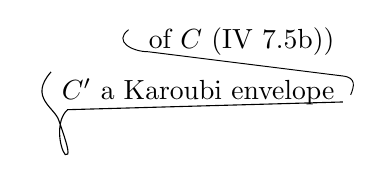
\begin{tikzpicture}[baseline=(kar.base),x=1cm,y=1cm]
\node[inner sep=0pt,anchor=base west] (kar) at (0,0) {$C'$ a Karoubi envelope};
\node[inner sep=0pt,anchor=base east] (ref) at ([yshift=.55cm]kar.east) {\inserted{of $C$ (IV 7.5\handwritten{b))}}};
\draw[line width=.4pt] (-.13,.35) .. controls (-.42,.02) and (-.08,-.10) .. (-.03,-.27)
 .. controls (.10,-.64) and (.11,-.72) .. (.05,-.70)
 .. controls (-.02,-.62) and (-.08,-.27) .. (.08,-.13)
 -- ([xshift=.10cm,yshift=-.13cm]kar.east);
\draw[line width=.35pt] ([xshift=-.25cm,yshift=.15cm]ref.west)
 .. controls ([xshift=-.45cm]ref.west) and ([xshift=-.20cm,yshift=-.13cm]ref.west)
 .. ([yshift=-.13cm]ref.west)
 -- ([xshift=.10cm,yshift=.20cm]kar.east)
 .. controls ([xshift=.28cm,yshift=.18cm]kar.east) and ([xshift=.24cm,yshift=.06cm]kar.east)
 .. ([xshift=.20cm,yshift=-.04cm]kar.east);
\end{tikzpicture}} Show that the following conditions are equivalent:

(i) The category $\mathrm{Ind}(C)$ (I 8.2) is a \uline{$U$}-topos.

( bis) The canonical functor $\mathrm{Ind}(C)\handwritten{\longrightarrow}\overset{\handwritten{\scriptscriptstyle\wedge}}{C}$ admits a right adjoint which \deleted{commutes with the} i\unsure{\deleted{n}s|\deleted{s}n} left ex\(\mathbb{a}\)ct.

(i ter) There exists a topology on $C$ for which the sheaves are the ind-representable presheaves.

\figure{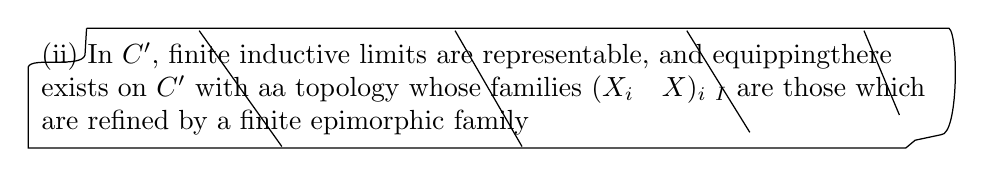
\begin{tikzpicture}
\node[inner sep=4pt,anchor=north west,text width=.94\linewidth] (oldii) at (0,0)
{\deleted{(ii) In $C'$, finite inductive limits are representable, \deleted{and equipping}\inserted{there exists on} $C'$ \deleted{\unsure{with a}}\inserted{a} topology whose families $(X_i\quad X)_{i\ I}$ are those which are refined by a finite epimorphic family}};
\draw[line width=.45pt] ([xshift=.72cm,yshift=.03cm]oldii.north west)
 -- ([xshift=-.02cm,yshift=.03cm]oldii.north east)
 .. controls ([xshift=.10cm,yshift=-.05cm]oldii.north east)
 and ([xshift=.10cm,yshift=.15cm]oldii.south east)
 .. ([xshift=-.12cm,yshift=.15cm]oldii.south east)
 -- ([xshift=-.45cm,yshift=.08cm]oldii.south east)
 -- ([xshift=-.57cm,yshift=-.02cm]oldii.south east)
 -- ([xshift=-.02cm,yshift=-.02cm]oldii.south west)
 -- ([xshift=-.02cm,yshift=-.46cm]oldii.north west)
 .. controls ([xshift=.02cm,yshift=-.33cm]oldii.north west)
 and ([xshift=.65cm,yshift=-.48cm]oldii.north west)
 .. ([xshift=.70cm,yshift=-.31cm]oldii.north west)
 -- ([xshift=.72cm,yshift=.03cm]oldii.north west);
\draw[line width=.45pt] ([xshift=2.15cm]oldii.north west)--([xshift=3.20cm]oldii.south west);
\draw[line width=.45pt] ([xshift=5.40cm]oldii.north west)--([xshift=6.25cm]oldii.south west);
\draw[line width=.45pt] ([xshift=-3.35cm]oldii.north east)--([xshift=-2.55cm,yshift=.18cm]oldii.south east);
\draw[line width=.45pt] ([xshift=-1.10cm]oldii.north east)--([xshift=-.65cm,yshift=.40cm]oldii.south east);
\end{tikzpicture}}

(ii) \deleted{In $C'$} Ther\begin{tikzpicture}[baseline=(ell.base),x=1em,y=1ex]
\node[inner sep=0pt,anchor=base] (ell) at (0,0) {e};
\draw[line width=.45pt] (-.19,2.05)--(.19,2.05)--(.19,2.35);
\draw[line width=.45pt] (-.19,-.40)--(.02,-.40)--(.02,-.72);
\end{tikzpicture} exists a topology on $C'$ whose cove\unsure{\deleted{a}r|\deleted{r}a}i\unsure{\deleted{t}n|\deleted{n}t}g families are those which a\unsure{\deleted{j}r|\deleted{r}j}e refined by a \uline{finite} epimorphic (or again, universally effective epimorphic ..) family, in $C'$ finite \deleted{projective}\inserted{inductive} limits are representable, and the canonical functor $C\handwritten{\longrightarrow}\overset{\handwritten{\scriptscriptstyle\sim}}{C}$ \deleted{is} commutes with them.

(iii) (If in $C$ finite projective limits are representab\deleted{\unsure{l|e}}le,\deleted{\unsure{â|à}} so that one can take $C'=C$.) In $C$ finite inductive limits are representable, and $C$ satisfies condition ST) of
\reversemarginpar\margin{\handwritten{$\times$}}\normalmarginpar
I 8.8 f).

(iv) There exists a topos $E$ generated by its full subcategory
\reversemarginpar\margin{\handwritten{$\times$}}\normalmarginpar
$E_{\mathrm{PF}}$ (\quad\quad), and an equivalence of categories $C'\handwritten{\approxeq}E_{\mathrm{PF}}$.

Moreover, \deleted{the topology} if these conditions are satisfied, the topology postulated in (i ter) is necessarily the one described in (ii), and the topos $E$ postulated in (iv) is necessarily equivalent to $\mathrm{Ind}(C)$. This topos is therefore perfect if and only if \inserted{in} $C'$ \deleted{is} finite projective limits are r\unsure{\deleted{r}e|\deleted{e}r}presentable.
% archive sheet number: 22
